\documentclass[12pt,aspectratio=169]{beamer}
\usepackage[T1]{fontenc}
\usepackage{lmodern,amsmath,amssymb,booktabs,tikz,graphicx}
\usetikzlibrary{arrows.meta,positioning,calc}
\definecolor{Ink}{HTML}{17324D}
\definecolor{Teal}{HTML}{007F7A}
\definecolor{Muted}{HTML}{556574}
\definecolor{Paper}{HTML}{FAFAF7}
\definecolor{Rust}{HTML}{AD532E}
\definecolor{Gold}{HTML}{B38630}
\setbeamercolor{background canvas}{bg=Paper}
\setbeamercolor{normal text}{fg=Ink}
\setbeamercolor{frametitle}{fg=Ink}
\setbeamercolor{structure}{fg=Teal}
\setbeamercolor{alerted text}{fg=Rust}
\setbeamerfont{frametitle}{size=\LARGE,series=\bfseries}
\setbeamertemplate{navigation symbols}{}
\setbeamersize{text margin left=9mm,text margin right=9mm}
\setbeamertemplate{frametitle}{\par\vspace{2mm}\insertframetitle\par\vspace{1mm}{\color{Gold}\rule{14mm}{1pt}}}
\setbeamertemplate{footline}{\hspace{9mm}\scriptsize\color{Muted}\insertsectionhead\hfill\insertframenumber\hspace{9mm}\vspace{4mm}}
\hypersetup{colorlinks=true,urlcolor=Teal,linkcolor=Muted,pdfauthor={}}
\newcommand{\point}[1]{\par\vspace{3mm}{\large #1\par}}
\newcommand{\eqnote}[1]{\par\vspace{2mm}{\small\color{Muted}#1\par}}
\newcommand{\smalltext}[1]{\eqnote{#1}}
\newcommand{\insight}[1]{\par\vspace{2mm}{\color{Teal}\bfseries #1}\par}
\newcommand{\identity}{\text{\scriptsize accounting identity}}
\newcommand{\policy}{R^{\mathrm{policy}}}
\newcommand{\loanrate}{R^{\mathrm{loan}}}
\newcommand{\nominal}{R^{\mathrm{nom}}}
\newcommand{\realrate}{R^{\mathrm{real}}}
\newcommand{\neutral}{R^{\mathrm{neutral}}}
\newcommand{\spot}[1]{R^{\mathrm{spot}}(#1)}
\newcommand{\forward}[2]{R^{\mathrm{forward}}(#1,#2)}
\newcommand{\bondyield}{R^{\mathrm{bond}}}
\newcommand{\bondrate}[1]{R^{\mathrm{bond}}(#1)}
\AtBeginDocument{\setlength{\abovedisplayskip}{5pt}\setlength{\belowdisplayskip}{5pt}\setlength{\abovedisplayshortskip}{3pt}\setlength{\belowdisplayshortskip}{3pt}}

\hypersetup{pdftitle={Economics and Finance for Mathematicians: Foreign exchange}}
\begin{document}

% Slide 1: Foreign exchange

\begin{frame}[plain]
{\color{Teal}\large ECONOMICS AND FINANCE\quad /\quad 04}\par\vspace{9mm}{\Huge\bfseries Foreign exchange}\par\vspace{7mm}{\Large How do returns, expectations and purchasing power price a currency?}
\end{frame}

% Slide 2: Today’s route

\begin{frame}{Today’s route}
\point{Fix the quote and compare covered and uncovered returns.}\point{Use purchasing power as a long-run benchmark.}\point{Combine sticky prices and asset-market equilibrium to explain overshooting.}
\end{frame}

% Slide 3: Currency quotes and contracts
\section[Currency quotes and contracts]{Currency quotes and contracts}
\begin{frame}[plain]
{\color{Gold}\large LECTURE 4}\par\vspace{9mm}{\Huge\bfseries Currency quotes and contracts}\par\vspace{7mm}{\Large What exactly are you buying when a currency strengthens?}
\end{frame}

% Slide 4: One quote convention throughout

\begin{frame}{One quote convention throughout}
\[E_t=\text{home currency units per one foreign unit}.\]\point{$E$ rises: the home currency depreciates.}\point{$E$ falls: the home currency appreciates.}
\end{frame}

% Slide 5: A quotation example

\begin{frame}{A quotation example}
\begin{center}\begin{tabular}{@{}lll@{}}\toprule \textbf{Quote} & \textbf{Before} & \textbf{After}\\\midrule JPY per USD & 150 & 135\\[2mm]
JPY cost of USD 1,000 & 150,000 & 135,000\\\bottomrule\end{tabular}\end{center}\point{The yen appreciates. One dollar buys fewer yen.}
\end{frame}

% Slide 6: Spot, forward and FX swap

\begin{frame}{Spot, forward and FX swap}
\begin{center}\begin{tabular}{@{}p{.25\textwidth}p{.68\textwidth}@{}}\toprule \textbf{Contract} & \textbf{Currency exchange dates}\\\midrule Spot & Near settlement at today’s agreed rate\\[2mm]
Forward & One future exchange at a rate agreed today\\[2mm]
FX swap & An exchange now and a reverse exchange later\\\bottomrule\end{tabular}\end{center}\eqnote{A forward FX rate is a contract price, not a promise about the later spot rate.}
\end{frame}

% Slide 7: Covered interest parity
\section[Covered interest parity]{Covered interest parity}
\begin{frame}[plain]
{\color{Gold}\large LECTURE 4}\par\vspace{9mm}{\Huge\bfseries Covered interest parity}\par\vspace{7mm}{\Large Can two locked currency routes pay different amounts?}
\end{frame}

% Slide 8: Two routes for the same home-currency payoff

\begin{frame}{Two routes for the same home-currency payoff}
\begin{center}
\begin{tikzpicture}[>=Stealth,every node/.style={font=\small,align=center,text width=3.5cm}]\node at (0.0,0){Home funds\\100};\node at (5.1,0){Foreign investment\\via spot E};\node at (10.2,0){Home proceeds\\via forward F};\draw[->,Teal,thick] (1.9,0)--(3.1999999999999997,0);\draw[->,Teal,thick] (7.0,0)--(8.299999999999999,0);\end{tikzpicture}\end{center}\point{Compare this hedged route with lending directly at home.}
\end{frame}

% Slide 9: The locked payoff equation

\begin{frame}{The locked payoff equation}
\[100(1+R^{\rm home})=\frac{100}{E}(1+R^{\rm foreign})F.\]\[\boxed{\frac{F}{E}=\frac{1+R^{\rm home}}{1+R^{\rm foreign}}.}\]\eqnote{Covered interest parity, one matched period and consistent conventions.}\eqnote{$R^{\rm home},R^{\rm foreign}$: matched-period rates. E: spot quote. F: forward quote.}
\end{frame}

% Slide 10: A complete covered-parity calculation

\begin{frame}{A complete covered-parity calculation}
\[E=0.90\;\text{EUR per USD},\quad R^{\rm EUR}=2\%,\quad R^{\rm USD}=5\%.\]\[F=0.90\frac{1.02}{1.05}=0.874286\;\text{EUR per USD}.\]\[100\;\text{EUR}\to111.111\;\text{USD}\to116.667\;\text{USD}\to102\;\text{EUR}.\]
\end{frame}

% Slide 11: Why covered parity can show a basis

\begin{frame}{Why covered parity can show a basis}
\point{Dealer balance sheets, collateral and funding are costly.}\point{The relevant borrowing rate can differ from the lending rate.}\point{A quoted pricing gap need not be a scalable free profit.}
\end{frame}

% Slide 12: Uncovered returns and carry
\section[Uncovered returns and carry]{Uncovered returns and carry}
\begin{frame}[plain]
{\color{Gold}\large LECTURE 4}\par\vspace{9mm}{\Huge\bfseries Uncovered returns and carry}\par\vspace{7mm}{\Large What changes when the future conversion rate is uncertain?}
\end{frame}

% Slide 13: The unhedged foreign payoff

\begin{frame}{The unhedged foreign payoff}
\[\text{Home-currency gross return}=(1+R^{\rm foreign})\frac{E_{t+1}}{E_t}.\]\point{$E_{t+1}$ is the future spot quote. It is unknown today.}
\end{frame}

% Slide 14: Uncovered interest parity is an equilibrium assumption

\begin{frame}{Uncovered interest parity is an equilibrium assumption}
\[R^{\rm home}\approx R^{\rm foreign}+\mathbb E_t\Delta\ln E_{t+1}.\]\point{Equal expected returns require assumptions about risk and beliefs.}
\end{frame}

% Slide 15: Currency risk premium

\begin{frame}{Currency risk premium}
\[R^{\rm home}-R^{\rm foreign}-\mathbb E_t\Delta\ln E_{t+1}=\rho_t.\]\point{$\rho_t$: expected excess return required on the home asset.}\point{The rate differential mixes expected FX change and compensation for risk.}
\end{frame}

% Slide 16: Carry: borrow yen and invest dollars

\begin{frame}{Carry: borrow yen and invest dollars}
\[E_t=150\;\text{JPY per USD},\quad R^{\rm JPY}=1\%,\quad R^{\rm USD}=5\%.\]\point{Borrow JPY 150 and buy USD 1.}\point{Next year receive USD 1.05 and owe JPY 151.50.}
\end{frame}

% Slide 17: A small interest gain can meet a large FX loss

\begin{frame}{A small interest gain can meet a large FX loss}
\begin{center}\begin{tabular}{@{}llll@{}}\toprule \textbf{Future JPY per USD} & \textbf{JPY proceeds} & \textbf{Debt due} & \textbf{P\&L}\\\midrule 150 & 157.50 & 151.50 & +6.00\\[2mm]
135 & 141.75 & 151.50 & -9.75\\\bottomrule\end{tabular}\end{center}\eqnote{In the second scenario, JPY per USD falls 10\%. Figures are hypothetical.}
\end{frame}

% Slide 18: The carry payoff depends on the exit exchange rate

\begin{frame}{The carry payoff depends on the exit exchange rate}
\begin{center}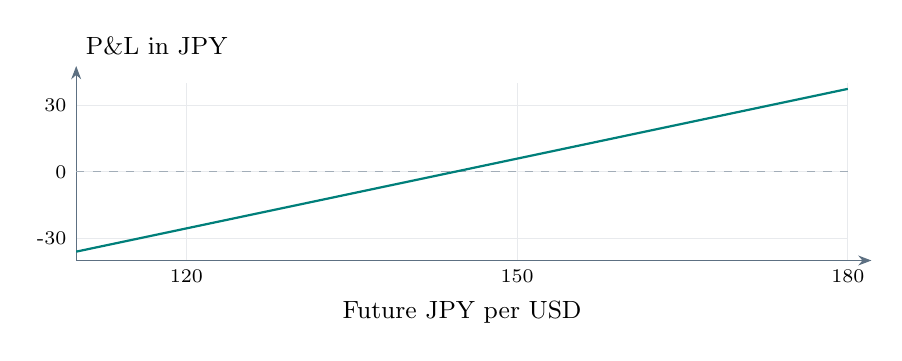
\begin{tikzpicture}[>=Stealth,every node/.style={font=\small}]
\draw[Ink!10] (1.4000,0.0000)--(1.4000,2.2500);\node[below,font=\scriptsize] at (1.4000,0.0000){120};
\draw[Ink!10] (5.6000,0.0000)--(5.6000,2.2500);\node[below,font=\scriptsize] at (5.6000,0.0000){150};
\draw[Ink!10] (9.8000,0.0000)--(9.8000,2.2500);\node[below,font=\scriptsize] at (9.8000,0.0000){180};
\draw[Ink!10] (0.0000,0.2812)--(9.8000,0.2812);\node[left,font=\scriptsize] at (0.0000,0.2812){-30};
\draw[Ink!10] (0.0000,1.1250)--(9.8000,1.1250);\node[left,font=\scriptsize] at (0.0000,1.1250){0};
\draw[Ink!10] (0.0000,1.9688)--(9.8000,1.9688);\node[left,font=\scriptsize] at (0.0000,1.9688){30};
\draw[->,Ink!70] (0,0)--(10.100000000000001,0);\draw[->,Ink!70] (0,0)--(0,2.47);
\node[below] at (4.9,-.40){Future JPY per USD};\node[anchor=west] at (0,2.73){P\&L in JPY};
\draw[Ink!40,dashed] (0.0000,1.1250)--(9.8000,1.1250);
\draw[Teal,thick] plot coordinates {(0.0000,0.1125) (0.1400,0.1420) (0.2800,0.1716) (0.4200,0.2011) (0.5600,0.2306) (0.7000,0.2602) (0.8400,0.2897) (0.9800,0.3192) (1.1200,0.3488) (1.2600,0.3783) (1.4000,0.4078) (1.5400,0.4373) (1.6800,0.4669) (1.8200,0.4964) (1.9600,0.5259) (2.1000,0.5555) (2.2400,0.5850) (2.3800,0.6145) (2.5200,0.6441) (2.6600,0.6736) (2.8000,0.7031) (2.9400,0.7327) (3.0800,0.7622) (3.2200,0.7917) (3.3600,0.8213) (3.5000,0.8508) (3.6400,0.8803) (3.7800,0.9098) (3.9200,0.9394) (4.0600,0.9689) (4.2000,0.9984) (4.3400,1.0280) (4.4800,1.0575) (4.6200,1.0870) (4.7600,1.1166) (4.9000,1.1461) (5.0400,1.1756) (5.1800,1.2052) (5.3200,1.2347) (5.4600,1.2642) (5.6000,1.2937) (5.7400,1.3233) (5.8800,1.3528) (6.0200,1.3823) (6.1600,1.4119) (6.3000,1.4414) (6.4400,1.4709) (6.5800,1.5005) (6.7200,1.5300) (6.8600,1.5595) (7.0000,1.5891) (7.1400,1.6186) (7.2800,1.6481) (7.4200,1.6777) (7.5600,1.7072) (7.7000,1.7367) (7.8400,1.7663) (7.9800,1.7958) (8.1200,1.8253) (8.2600,1.8548) (8.4000,1.8844) (8.5400,1.9139) (8.6800,1.9434) (8.8200,1.9730) (8.9600,2.0025) (9.1000,2.0320) (9.2400,2.0616) (9.3800,2.0911) (9.5200,2.1206) (9.6600,2.1502) (9.8000,2.1797)};
\end{tikzpicture}\end{center}\eqnote{Break-even: 151.50 / 1.05 = 144.29 JPY per USD, before costs.}
\end{frame}

% Slide 19: Crash risk can hide behind frequent small gains

\begin{frame}{Crash risk can hide behind frequent small gains}
\begin{center}\begin{tabular}{@{}lll@{}}\toprule \textbf{Toy outcome} & \textbf{Probability} & \textbf{Normalised P\&L}\\\midrule Quiet period & 95\% & +4\%\\[2mm]
Funding-currency surge & 5\% & -60\%\\\bottomrule\end{tabular}\end{center}\[0.95(4\%)+0.05(-60\%)=0.8\%.\]\eqnote{An invented distribution, not an estimate of any currency strategy.}
\end{frame}

% Slide 20: Expectations and purchasing power
\section[Expectations and purchasing power]{Expectations and purchasing power}
\begin{frame}[plain]
{\color{Gold}\large LECTURE 4}\par\vspace{9mm}{\Huge\bfseries Expectations and purchasing power}\par\vspace{7mm}{\Large Why can a rate increase mean appreciation now or weakness over time?}
\end{frame}

% Slide 21: Short-run FX as an asset price

\begin{frame}{Short-run FX as an asset price}
\[E_t=\frac{(1+R^{\rm foreign})E_t^e}{1+R^{\rm home}}.\]\point{$E_t^e$: expected next-period quote, fixed for this experiment.}\point{A higher home rate then supports a stronger home currency.}
\end{frame}

% Slide 22: A short-run FX return diagram

\begin{frame}{A short-run FX return diagram}
\begin{center}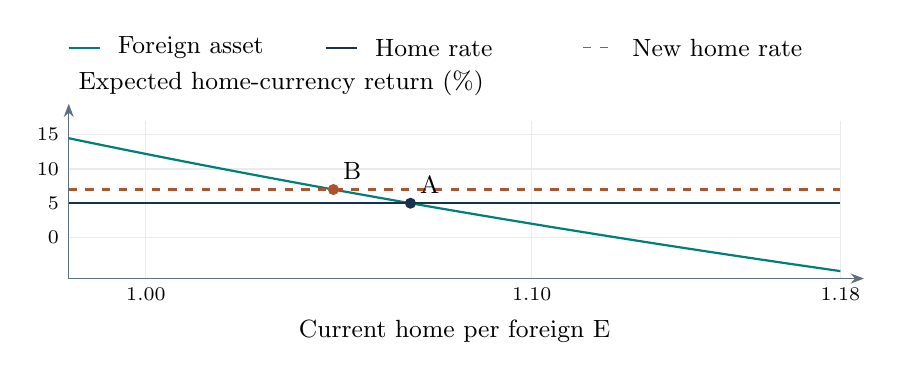
\begin{tikzpicture}[>=Stealth,every node/.style={font=\small}]
\draw[Ink!10] (0.9800,0.0000)--(0.9800,2.0000);\node[below,font=\scriptsize] at (0.9800,0.0000){1.00};
\draw[Ink!10] (5.8800,0.0000)--(5.8800,2.0000);\node[below,font=\scriptsize] at (5.8800,0.0000){1.10};
\draw[Ink!10] (9.8000,0.0000)--(9.8000,2.0000);\node[below,font=\scriptsize] at (9.8000,0.0000){1.18};
\draw[Ink!10] (0.0000,0.5217)--(9.8000,0.5217);\node[left,font=\scriptsize] at (0.0000,0.5217){0};
\draw[Ink!10] (0.0000,0.9565)--(9.8000,0.9565);\node[left,font=\scriptsize] at (0.0000,0.9565){5};
\draw[Ink!10] (0.0000,1.3913)--(9.8000,1.3913);\node[left,font=\scriptsize] at (0.0000,1.3913){10};
\draw[Ink!10] (0.0000,1.8261)--(9.8000,1.8261);\node[left,font=\scriptsize] at (0.0000,1.8261){15};
\draw[->,Ink!70] (0,0)--(10.100000000000001,0);\draw[->,Ink!70] (0,0)--(0,2.22);
\node[below] at (4.9,-.40){Current home per foreign E};\node[anchor=west] at (0,2.48){Expected home-currency return (\%)};
\draw[Teal,thick] plot coordinates {(0.0000,1.7817) (0.0980,1.7614) (0.1960,1.7413) (0.2940,1.7211) (0.3920,1.7011) (0.4900,1.6812) (0.5880,1.6613) (0.6860,1.6415) (0.7840,1.6218) (0.8820,1.6022) (0.9800,1.5826) (1.0780,1.5631) (1.1760,1.5437) (1.2740,1.5244) (1.3720,1.5052) (1.4700,1.4860) (1.5680,1.4669) (1.6660,1.4479) (1.7640,1.4290) (1.8620,1.4101) (1.9600,1.3913) (2.0580,1.3726) (2.1560,1.3539) (2.2540,1.3354) (2.3520,1.3169) (2.4500,1.2984) (2.5480,1.2801) (2.6460,1.2618) (2.7440,1.2436) (2.8420,1.2254) (2.9400,1.2074) (3.0380,1.1894) (3.1360,1.1714) (3.2340,1.1535) (3.3320,1.1357) (3.4300,1.1180) (3.5280,1.1003) (3.6260,1.0827) (3.7240,1.0652) (3.8220,1.0478) (3.9200,1.0304) (4.0180,1.0130) (4.1160,0.9958) (4.2140,0.9785) (4.3120,0.9614) (4.4100,0.9443) (4.5080,0.9273) (4.6060,0.9104) (4.7040,0.8935) (4.8020,0.8767) (4.9000,0.8599) (4.9980,0.8432) (5.0960,0.8266) (5.1940,0.8100) (5.2920,0.7935) (5.3900,0.7770) (5.4880,0.7606) (5.5860,0.7443) (5.6840,0.7280) (5.7820,0.7118) (5.8800,0.6957) (5.9780,0.6796) (6.0760,0.6635) (6.1740,0.6475) (6.2720,0.6316) (6.3700,0.6157) (6.4680,0.5999) (6.5660,0.5842) (6.6640,0.5685) (6.7620,0.5529) (6.8600,0.5373) (6.9580,0.5217) (7.0560,0.5063) (7.1540,0.4908) (7.2520,0.4755) (7.3500,0.4602) (7.4480,0.4449) (7.5460,0.4297) (7.6440,0.4146) (7.7420,0.3995) (7.8400,0.3844) (7.9380,0.3695) (8.0360,0.3545) (8.1340,0.3396) (8.2320,0.3248) (8.3300,0.3100) (8.4280,0.2953) (8.5260,0.2806) (8.6240,0.2660) (8.7220,0.2514) (8.8200,0.2369) (8.9180,0.2224) (9.0160,0.2080) (9.1140,0.1936) (9.2120,0.1793) (9.3100,0.1650) (9.4080,0.1508) (9.5060,0.1366) (9.6040,0.1224) (9.7020,0.1084) (9.8000,0.0943)};
\draw[Ink,thick] plot coordinates {(0.0000,0.9565) (9.8000,0.9565)};
\draw[Rust,dashed,thick] plot coordinates {(0.0000,1.1304) (9.8000,1.1304)};
\fill[Ink] (4.3400,0.9565) circle (2pt);\node[above right] at (4.3400,0.9565){A};
\fill[Rust] (3.3613,1.1304) circle (2pt);\node[above right] at (3.3613,1.1304){B};
\draw[Teal,thick] (0.0,2.93)--(0.4,2.93);\node[anchor=west,font=\small] at (0.5,2.93){Foreign asset};
\draw[Ink,thick] (3.266666666666667,2.93)--(3.666666666666667,2.93);\node[anchor=west,font=\small] at (3.766666666666667,2.93){Home rate};
\draw[Rust,dashed] (6.533333333333334,2.93)--(6.9333333333333345,2.93);\node[anchor=west,font=\small] at (7.033333333333334,2.93){New home rate};
\end{tikzpicture}\end{center}\eqnote{Expected future E = 1.10 and foreign rate 2\%, both fixed. Hypothetical values.}
\end{frame}

% Slide 23: The rate and expectation experiments

\begin{frame}{The rate and expectation experiments}
\begin{center}\begin{tabular}{@{}ll@{}}\toprule \textbf{Change, other inputs fixed} & \textbf{Current home-per-foreign E}\\\midrule Home interest rate rises & Falls: home appreciates\\[2mm]
Expected future E rises & Rises: home depreciates\\[2mm]
Required home risk premium rises & Rises: home weakens\\\bottomrule\end{tabular}\end{center}\eqnote{The third result uses the premium convention defined earlier.}
\end{frame}

% Slide 24: Purchasing power parity

\begin{frame}{Purchasing power parity}
\[E^{PPP}=\frac{Q^{\rm home}}{Q^{\rm foreign}}.\]\point{A comparable basket costs 100 at home and 80 abroad.}\point{PPP implies 1.25 home units per foreign unit.}
\end{frame}

% Slide 25: Why a cheap haircut is hard to arbitrage

\begin{frame}{Why a cheap haircut is hard to arbitrage}
\point{Haircuts require local labour and premises.}\point{National baskets have different weights and taxes.}\point{Productivity can change equilibrium relative prices.}
\end{frame}

% Slide 26: Productivity and local service prices

\begin{frame}{Productivity and local service prices}
\begin{center}\begin{tabular}{@{}llll@{}}\toprule \textbf{Toy economy} & \textbf{Tradable productivity} & \textbf{Wage} & \textbf{Haircut cost}\\\midrule A & 10 units / hour & 10 / hour & 10\\[2mm]
B & 5 units / hour & 5 / hour & 5\\\bottomrule\end{tabular}\end{center}\eqnote{Tradable price 1 in both economies. One haircut per hour. Mobile domestic labour.}
\end{frame}

% Slide 27: The real exchange rate

\begin{frame}{The real exchange rate}
\[q=\frac{E Q^{\rm foreign}}{Q^{\rm home}}.\]\point{$q$: foreign-basket price relative to the home basket.}\point{A rise in q is a real depreciation of the home currency.}
\end{frame}

% Slide 28: Relative PPP and the Fisher effect

\begin{frame}{Relative PPP and the Fisher effect}
\[\Delta\ln E\approx\pi^{\rm home}-\pi^{\rm foreign}.\]\point{Persistent higher home inflation tends to erode the home currency.}\point{Its higher nominal rate may simply compensate for that inflation.}
\end{frame}

% Slide 29: Real interest differences and real FX expectations

\begin{frame}{Real interest differences and real FX expectations}
\[R^{\rm real,home}-R^{\rm real,foreign}\approx\mathbb E_t\Delta\ln q+\rho_t.\]\point{Equal real rates need additional assumptions.}\point{Expected real FX changes and risk premia can support persistent differences.}
\end{frame}

% Slide 30: Dornbusch overshooting
\section[Dornbusch overshooting]{Dornbusch overshooting}
\begin{frame}[plain]
{\color{Gold}\large LECTURE 4}\par\vspace{9mm}{\Huge\bfseries Dornbusch overshooting}\par\vspace{7mm}{\Large Why can the currency jump further than its long-run adjustment?}
\end{frame}

% Slide 31: A permanent monetary level shock

\begin{frame}{A permanent monetary level shock}
\point{The money stock rises permanently by 10\% in the classic model.}\point{Prices are sticky initially. Long-run output is fixed.}\point{Flexible asset prices respond immediately.}
\end{frame}

% Slide 32: Prices adjust slowly

\begin{frame}{Prices adjust slowly}
\begin{center}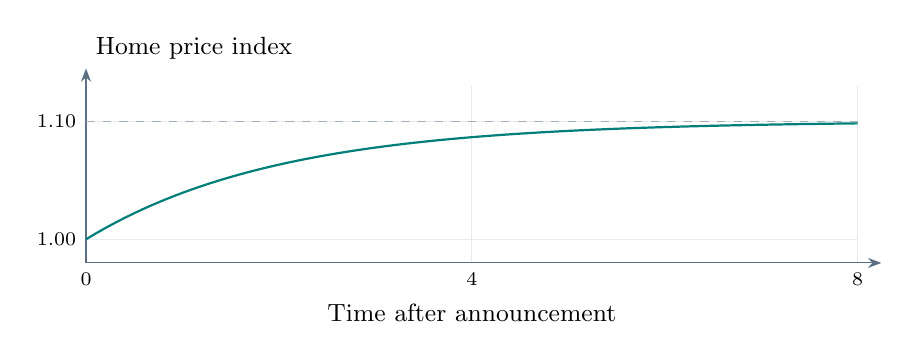
\begin{tikzpicture}[>=Stealth,every node/.style={font=\small}]
\draw[Ink!10] (0.0000,0.0000)--(0.0000,2.2500);\node[below,font=\scriptsize] at (0.0000,0.0000){0};
\draw[Ink!10] (4.9000,0.0000)--(4.9000,2.2500);\node[below,font=\scriptsize] at (4.9000,0.0000){4};
\draw[Ink!10] (9.8000,0.0000)--(9.8000,2.2500);\node[below,font=\scriptsize] at (9.8000,0.0000){8};
\draw[Ink!10] (0.0000,0.3000)--(9.8000,0.3000);\node[left,font=\scriptsize] at (0.0000,0.3000){1.00};
\draw[Ink!10] (0.0000,1.8000)--(9.8000,1.8000);\node[left,font=\scriptsize] at (0.0000,1.8000){1.10};
\draw[->,Ink!70] (0,0)--(10.100000000000001,0);\draw[->,Ink!70] (0,0)--(0,2.47);
\node[below] at (4.9,-.40){Time after announcement};\node[anchor=west] at (0,2.73){Home price index};
\draw[Ink!40,dashed] (0.0000,1.8000)--(9.8000,1.8000);
\draw[Teal,thick] plot coordinates {(0.0000,0.3000) (0.1225,0.3732) (0.2450,0.4427) (0.3675,0.5089) (0.4900,0.5719) (0.6125,0.6318) (0.7350,0.6888) (0.8575,0.7430) (0.9800,0.7945) (1.1025,0.8436) (1.2250,0.8902) (1.3475,0.9346) (1.4700,0.9768) (1.5925,1.0169) (1.7150,1.0551) (1.8375,1.0915) (1.9600,1.1260) (2.0825,1.1589) (2.2050,1.1901) (2.3275,1.2199) (2.4500,1.2482) (2.5725,1.2751) (2.6950,1.3007) (2.8175,1.3250) (2.9400,1.3482) (3.0625,1.3702) (3.1850,1.3912) (3.3075,1.4111) (3.4300,1.4301) (3.5525,1.4481) (3.6750,1.4653) (3.7975,1.4816) (3.9200,1.4972) (4.0425,1.5119) (4.1650,1.5260) (4.2875,1.5393) (4.4100,1.5521) (4.5325,1.5641) (4.6550,1.5756) (4.7775,1.5866) (4.9000,1.5970) (5.0225,1.6069) (5.1450,1.6163) (5.2675,1.6253) (5.3900,1.6338) (5.5125,1.6419) (5.6350,1.6496) (5.7575,1.6569) (5.8800,1.6639) (6.0025,1.6706) (6.1250,1.6769) (6.2475,1.6829) (6.3700,1.6886) (6.4925,1.6940) (6.6150,1.6992) (6.7375,1.7041) (6.8600,1.7088) (6.9825,1.7132) (7.1050,1.7175) (7.2275,1.7215) (7.3500,1.7253) (7.4725,1.7290) (7.5950,1.7324) (7.7175,1.7357) (7.8400,1.7389) (7.9625,1.7418) (8.0850,1.7447) (8.2075,1.7474) (8.3300,1.7499) (8.4525,1.7524) (8.5750,1.7547) (8.6975,1.7569) (8.8200,1.7590) (8.9425,1.7610) (9.0650,1.7629) (9.1875,1.7647) (9.3100,1.7664) (9.4325,1.7681) (9.5550,1.7696) (9.6775,1.7711) (9.8000,1.7725)};
\end{tikzpicture}\end{center}\eqnote{Original illustrative transition. Initial level 1, long-run level 1.10.}
\end{frame}

% Slide 33: The exchange rate can overshoot

\begin{frame}{The exchange rate can overshoot}
\begin{center}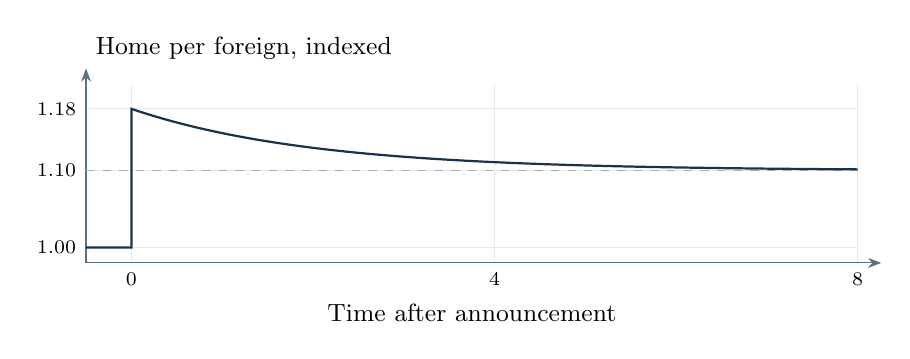
\begin{tikzpicture}[>=Stealth,every node/.style={font=\small}]
\draw[Ink!10] (0.5765,0.0000)--(0.5765,2.2500);\node[below,font=\scriptsize] at (0.5765,0.0000){0};
\draw[Ink!10] (5.1882,0.0000)--(5.1882,2.2500);\node[below,font=\scriptsize] at (5.1882,0.0000){4};
\draw[Ink!10] (9.8000,0.0000)--(9.8000,2.2500);\node[below,font=\scriptsize] at (9.8000,0.0000){8};
\draw[Ink!10] (0.0000,0.1957)--(9.8000,0.1957);\node[left,font=\scriptsize] at (0.0000,0.1957){1.00};
\draw[Ink!10] (0.0000,1.1739)--(9.8000,1.1739);\node[left,font=\scriptsize] at (0.0000,1.1739){1.10};
\draw[Ink!10] (0.0000,1.9565)--(9.8000,1.9565);\node[left,font=\scriptsize] at (0.0000,1.9565){1.18};
\draw[->,Ink!70] (0,0)--(10.100000000000001,0);\draw[->,Ink!70] (0,0)--(0,2.47);
\node[below] at (4.9,-.40){Time after announcement};\node[anchor=west] at (0,2.73){Home per foreign, indexed};
\draw[Ink!40,dashed] (0.0000,1.1739)--(9.8000,1.1739);
\draw[Ink,thick] plot coordinates {(0.0000,0.1957) (0.5765,0.1957) (0.5765,1.9565) (0.6918,1.9184) (0.8071,1.8820) (0.9224,1.8475) (1.0376,1.8147) (1.1529,1.7834) (1.2682,1.7537) (1.3835,1.7254) (1.4988,1.6985) (1.6141,1.6729) (1.7294,1.6486) (1.8447,1.6254) (1.9600,1.6034) (2.0753,1.5825) (2.1906,1.5625) (2.3059,1.5436) (2.4212,1.5256) (2.5365,1.5084) (2.6518,1.4921) (2.7671,1.4766) (2.8824,1.4618) (2.9976,1.4478) (3.1129,1.4344) (3.2282,1.4217) (3.3435,1.4096) (3.4588,1.3981) (3.5741,1.3872) (3.6894,1.3768) (3.8047,1.3669) (3.9200,1.3575) (4.0353,1.3485) (4.1506,1.3400) (4.2659,1.3319) (4.3812,1.3242) (4.4965,1.3169) (4.6118,1.3099) (4.7271,1.3033) (4.8424,1.2970) (4.9576,1.2910) (5.0729,1.2853) (5.1882,1.2798) (5.3035,1.2747) (5.4188,1.2697) (5.5341,1.2651) (5.6494,1.2606) (5.7647,1.2564) (5.8800,1.2524) (5.9953,1.2485) (6.1106,1.2449) (6.2259,1.2414) (6.3412,1.2382) (6.4565,1.2350) (6.5718,1.2320) (6.6871,1.2292) (6.8024,1.2265) (6.9176,1.2239) (7.0329,1.2215) (7.1482,1.2192) (7.2635,1.2170) (7.3788,1.2149) (7.4941,1.2129) (7.6094,1.2110) (7.7247,1.2092) (7.8400,1.2074) (7.9553,1.2058) (8.0706,1.2043) (8.1859,1.2028) (8.3012,1.2014) (8.4165,1.2000) (8.5318,1.1988) (8.6471,1.1975) (8.7624,1.1964) (8.8776,1.1953) (8.9929,1.1943) (9.1082,1.1933) (9.2235,1.1923) (9.3388,1.1914) (9.4541,1.1906) (9.5694,1.1898) (9.6847,1.1890) (9.8000,1.1882)};
\end{tikzpicture}\end{center}\eqnote{The home currency weakens sharply, then appreciates toward its new long-run level.}
\end{frame}

% Slide 34: The overshooting mechanism

\begin{frame}{The overshooting mechanism}
\begin{center}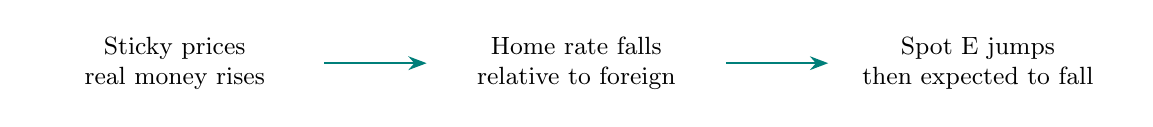
\begin{tikzpicture}[>=Stealth,every node/.style={font=\small,align=center,text width=3.5cm}]\node at (0.0,0){Sticky prices\\real money rises};\node at (5.1,0){Home rate falls\\relative to foreign};\node at (10.2,0){Spot E jumps\\then expected to fall};\draw[->,Teal,thick] (1.9,0)--(3.1999999999999997,0);\draw[->,Teal,thick] (7.0,0)--(8.299999999999999,0);\end{tikzpicture}\end{center}\point{An expected future appreciation reconciles the lower home interest rate.}
\end{frame}

% Slide 35: Exercise: three explanations for a high yield

\begin{frame}{Exercise: three explanations for a high yield}
\point{Case A: an unexpected tightening, fixed future inflation and FX expectations.}\point{Case B: higher expected persistent inflation.}\point{Case C: a larger currency risk premium.}
\end{frame}

% Slide 36: Further reading
\section[Reading]{Reading}
\begin{frame}{Further reading}
\point{Dmitriy Sergeyev, Bocconi 30054 course materials.}\point{Krugman, Obstfeld \& Melitz, \emph{International Economics}.}\point{Source links and worked answers accompany each slide in the notes.}
\end{frame}
\end{document}
